% !TEX TS-program = pdflatex
% !TeX program = pdflatex
% !TEX encoding = UTF-8
% !TEX spellcheck = fr

\documentclass{beamer}
%\usepackage{fullpage}
%\usepackage[left=2.8cm,right=2.2cm,top=2 cm,bottom=2 cm]{geometry}
\setbeamersize{text margin left=10pt,text margin right=10pt}
\usepackage{amsmath,amssymb} 
\usepackage[T1]{fontenc}
\usepackage[utf8]{inputenc}
\usepackage[english,french]{babel}
\usepackage{txfonts}
\usepackage[]{graphicx}
\usepackage{multirow}
\usepackage{hyperref}
\usepackage{listings}


\hypersetup{
	colorlinks,
	urlcolor = blue
}

%\renewcommand{\baselinestretch}{1.5}

\def\supit#1{\raisebox{0.8ex}{\small\it #1}\hspace{0.05em}}



\AtBeginSection{%
	\begin{frame}
		\sectionpage
	\end{frame}
}

\newcommand{\rottext}[2]{%
	\rotatebox{90}{%
	\begin{minipage}{#1}%
		\raggedleft#2%
	\end{minipage}%
	}%
}

\usepackage{longtable}
\usepackage{tabu}


\title[BWEB: 01- RI et Gmail] %
{Bureautique et Web \\Chapitre 02: Recherche d'information et messagerie} 
\institute{ %
École  nationale Supérieure d'Informatique (ESI, ex. INI), Algérie
}
\author[ \textbf{\footnotesize  \insertframenumber/\inserttotalframenumber} \hspace*{1cm} ESI - ARIES Abdelkrime (2019-2020)] %
{ARIES Abdelkrime}
%\titlegraphic{
\includegraphics[height=1cm]{../img/esi-logo.png}%\hspace*{4.75cm}~


\date{Année unniversitaire: 2019/2020} %\today

\usetheme{Warsaw} % Antibes Boadilla Warsaw

\beamertemplatenavigationsymbolsempty

%\setbeamertemplate{headline}{}


\begin{document}
	
	\newcolumntype{L}[2]{%
		>{\vbox to #2\bgroup\vfill\flushleft}%
		p{#1}%
		<{\egroup}} 

\begin{frame}[plain]
	\maketitle
\end{frame}

\section{Recherche d'information}

\begin{frame}
\frametitle{Recherche d'information}

%Pour préparer un rapport ou une présentation: 
%\begin{itemize}
%	\item Cerner le sujet 
%	\item Localiser l'information 
%	\item Collecter les informations 
%	\item Traiter l'information 
%	\item Restituer l'information 
%	\item Rédiger le travail
%\end{itemize} 

\includegraphics[height=.9\textheight]{..//img/Bweb02-ri-gmail/etapes-rapport.pdf}


\end{frame}

\begin{frame}
\frametitle{Recherche d'information}

Afin de localiser l'information: 
\begin{itemize}
	\item Exploration des ressources 
	\item Recherche par mots clés
\end{itemize} 

\end{frame}

\subsection{Moteurs de recherche}

\begin{frame}
\frametitle{Recherche d'information}
\frametitle{Moteurs de recherche}

\end{frame}

\begin{frame}
\frametitle{Recherche d'information}
\frametitle{Moteur de recherche}

\end{frame}


\begin{frame}
\frametitle{Recherche d'information}
\framesubtitle{Quelque moteurs de recherche web (génériques)}

\def\arraystretch{0}

\begin{tabular}{L{.3\textwidth}{.8cm}cp{.6\textwidth}}%p{.3\textwidth}
	
	\hline
	
	
\includegraphics[height=.8cm]{..//img/Bweb02-ri-gmail/google-logo.png} &
	& 
	\url{https://www.google.com/}  \\
	
	\hline
	
	
\includegraphics[height=.8cm]{..//img/Bweb02-ri-gmail/bing-logo.png} &
	& 
	\url{https://www.bing.com/} \\
	
	\hline
	
	
\includegraphics[height=.4cm]{..//img/Bweb02-ri-gmail/yahoo-logo.png} & 
	& 
	\url{https://search.yahoo.com/} \\
	
	\hline
	
	
\includegraphics[height=.8cm]{..//img/Bweb02-ri-gmail/baidu-logo.png} & 
	& 
	\url{https://www.baidu.com/} \\
	
	\hline
	
	
\includegraphics[height=.8cm]{..//img/Bweb02-ri-gmail/yandex-logo.png} & 
	& 
	\url{https://yandex.com/} \\
	
	\hline
	
\end{tabular}

%\begin{itemize}
%	\item Google
%	\item Bing 
%	\item Yahoo
%	\item DuckDuckGo
%\end{itemize}

\end{frame}


\begin{frame}
\frametitle{Recherche d'information}
\framesubtitle{Quelque moteurs de recherche académique}

%\begin{tabular}{p{.4\textwidth}cp{.4\textwidth}}
%	Google Scholar && Microsoft Academic \\
%	\url{https://scholar.google.com/} && \url{https://academic.microsoft.com/}  \\
%	
\includegraphics[height=1cm]{..//img/Bweb02-ri-gmail/gscholar-logo.png} && 
%	
\includegraphics[height=1cm]{..//img/Bweb02-ri-gmail/msacademic-logo.jpg} \\
%	&& \\ 
%	
%	BASE && CORE \\
%	\url{https://www.base-search.net/} && \url{https://core.ac.uk/}  \\
%	
\includegraphics[height=1cm]{..//img/Bweb02-ri-gmail/base-logo.png} && 
%	
\includegraphics[height=1cm]{..//img/Bweb02-ri-gmail/core-logo.png} \\
%	
%\end{tabular}

\def\arraystretch{0}
\begin{tabular}{L{.3\textwidth}{1cm}cp{.6\textwidth}}%p{.3\textwidth}
	
	\hline
	
	
\includegraphics[height=.6cm]{..//img/Bweb02-ri-gmail/gscholar-logo.png} &
	&
	\url{https://scholar.google.com/} \\
	
	\hline
	
	
\includegraphics[height=1cm]{..//img/Bweb02-ri-gmail/msacademic-logo.png} &
	& 
	\url{https://academic.microsoft.com/}  \\
	
	\hline
	
	
\includegraphics[height=1cm]{..//img/Bweb02-ri-gmail/base-logo.png} &
	& 
	\url{https://www.base-search.net/} \\
	
	\hline
	
	
\includegraphics[height=1cm]{..//img/Bweb02-ri-gmail/core-logo.png} & 
	& 
	\url{https://core.ac.uk/} \\
	
	\hline
	
\end{tabular}

%\begin{itemize}
%	\item Google Scholar 
%	\item Microsoft Academic
%	\item BASE
%	\item CORE
%\end{itemize}

\end{frame}


\begin{frame}
\frametitle{Recherche d'information}
\framesubtitle{Quelque bibliothèques de recherche d'information}

\begin{tabular}{p{.3\textwidth}cp{.6\textwidth}}
	
	\hline
	
	
\includegraphics[height=.8cm]{..//img/Bweb02-ri-gmail/solr-logo.png} &
	& 
	\url{https://academic.microsoft.com/}  \\
	
	\hline
	
	
\includegraphics[height=.8cm]{..//img/Bweb02-ri-gmail/elastic-logo.png} &
	& 
	\url{https://www.elastic.co/products/elasticsearch} \\
	
	\hline
	
	
\includegraphics[height=.8cm]{..//img/Bweb02-ri-gmail/sphinx-logo.png} & 
	& 
	\url{http://sphinxsearch.com/} \\
	
	\hline
	
	
\includegraphics[height=.8cm]{..//img/Bweb02-ri-gmail/xapian-logo.png} & 
	& 
	\url{https://core.ac.uk/} \\
	
	\hline
	
\end{tabular}

%\begin{itemize}
%	\item Lucene
%	\item Solr 
%	\item Elasticsearch
%	\item Sphinx
%	\item Xapian
%\end{itemize}

\end{frame}

\begin{frame}
\frametitle{Recherche d'information}
\framesubtitle{Quelque moteurs de recherche de bureau}

\begin{tabular}{p{.3\textwidth}cp{.6\textwidth}}
	
	\hline
	
	
\includegraphics[height=.8cm]{..//img/Bweb02-ri-gmail/solr-logo.png} &
	& 
	\url{https://academic.microsoft.com/}  \\
	
	\hline
	
	
\includegraphics[height=.8cm]{..//img/Bweb02-ri-gmail/elastic-logo.png} &
	& 
	\url{https://www.elastic.co/products/elasticsearch} \\
	
	\hline
	
	
\includegraphics[height=.8cm]{..//img/Bweb02-ri-gmail/sphinx-logo.png} & 
	& 
	\url{http://sphinxsearch.com/} \\
	
	\hline
	
	
\includegraphics[height=.8cm]{..//img/Bweb02-ri-gmail/xapian-logo.png} & 
	& 
	\url{https://core.ac.uk/} \\
	
	\hline
	
\end{tabular}

%\begin{itemize}
%	\item Lucene
%	\item Solr 
%	\item Elasticsearch
%	\item Sphinx
%	\item Xapian
%\end{itemize}

\end{frame}

\subsection{Structure d'un moteur de recherche}

\begin{frame}
\frametitle{Recherche d'information}
\framesubtitle{Structure d'un moteur de recherche}

\begin{center}
	\includegraphics[height=.87\textheight]{..//img/Bweb02-ri-gmail/moteur-recherche.pdf}
\end{center}
%\begin{itemize}
%	\item indexation 
%	\begin{itemize}
%		\item Acquisition (Exploration et ...)
%		\item Transformation 
%		\item Création d'index
%	\end{itemize}
%	\item interrogation
%	\begin{itemize}
%		\item Interaction avec l'utilisateur
%		\item Classement 
%		\item Évaluation
%	\end{itemize}
%\end{itemize}

\end{frame}

\begin{frame}
\frametitle{Recherche d'information: Structure}
\framesubtitle{Acquisition}

\begin{itemize}
	\item Exploration; un explorateur (robot, spider, crawler)
	\begin{itemize}
		\item parcourt les sites web périodiquement 
		\item suit les liens hypertextes pour trouver des documents
	\end{itemize}

	\item Conversion:
	\begin{itemize}
		\item vers du texte; il existe des formats de fichiers non textuels (ex. PDF, Word, etc.)
		\item vers un encodage standard (ex. UTF-8)
	\end{itemize}
\end{itemize}

\end{frame}

\begin{frame}
\frametitle{Recherche d'information: Structure}
\framesubtitle{Exploration: points négatifs}

Les explorateurs (spiders) ont quelques points négatifs; ils:
\begin{itemize}
	\item peuvent télécharger des informations privées ou classifiées
	\item ne prennent pas en considération les termes d'utilisation des sites web. 
	Par exemple, un site web qui donne droit de lecture sans recopier les informations. 
	\item surchargent les serveurs par des requêtes, ce qui entraine leur plantage ou les rend lourds.
\end{itemize}

\end{frame}

\begin{frame}[fragile]
\frametitle{Recherche d'information}
\framesubtitle{Exploration: Bloquer l'accès à votre contenu}

% https://support.google.com/webmasters/answer/6062608?hl=fr

En créant un fichier texte "\textbf{robot.txt}" dans la racine de votre site web, on peut bloquer des agents (robots) d'exploration.

%\begin{block}{Syntaxe simple de "robot.txt"}
%	\scriptsize\bfseries
%	\begin{lstlisting}
%	# commentaire
%	User-agent: [nom d'agent]
%	Disallow: [URL de ce qu'on veut bloquer] 
%	
%	# il faut laisser une ligne vide pour un autre groupe
%	\end{lstlisting}
%\end{block}

\begin{exampleblock}{exemple d'un fichier "robot.txt"}
	\scriptsize\bfseries
	\begin{lstlisting}
	# empecher Google a explorer un dossier et un fichier
	User-agent: Googlebot
	Disallow: /spam/ 
	Disallow: /utilisateurs.html
	
	# empecher Google a explorer les fichiers .doc 
	User-agent: Bingbot
	Disallow: /*.doc$ 
	
	# empecher tous les agents a explorer un dossier
	User-agent: *
	Disallow: /prive/
	\end{lstlisting}
\end{exampleblock}


\end{frame}

\begin{frame}[fragile]
\frametitle{Recherche d'information}
\framesubtitle{Exploration: Bloquer l'accès à votre contenu}

% https://developers.google.com/search/reference/robots_meta_tag
En l'indiquant dans le code HTML de vos pages

\begin{exampleblock}{exemple d'un fichier HTML qui bloque tous les robots}
	\scriptsize\bfseries
	\begin{lstlisting}
	<!DOCTYPE html>
	<html>
	    <head>
	        <meta name="robots" content="noindex" />
	    </head>
	    <body>
	    </body>
	</html>
	\end{lstlisting}
\end{exampleblock}

\begin{exampleblock}{exemple d'un meta qui bloque Google}
	\scriptsize\bfseries
	\begin{lstlisting}
	<meta name="googlebot" content="noindex" />
	\end{lstlisting}
\end{exampleblock}

\end{frame}

\begin{frame}
\frametitle{Recherche d'information: Structure}
\framesubtitle{Transformation}

\begin{itemize}
	\item Segmentation du texte vers des mots. 
	Exemple, \textcolor{red}{"Je suis une formation en BWeb" --> [Je, suis, une, formation, en, BWeb]}
	
	\item Suppression des mots vides (prépositions, articles, pronoms, etc.)
	Exemple, \textcolor{red}{[Je, suis, une, formation, en, BWeb] --> [suis, formation, BWeb]}
	
	\item Radicalisation (stemming): suppression des préfixes, suffixes et infixes. 
	Exemple, \textcolor{red}{formation --> form}
\end{itemize}

\end{frame}

\begin{frame}
\frametitle{Recherche d'information: Structure}
\framesubtitle{Création d'index}

\begin{itemize}
	\item Faire des statistiques sur les documents. 
	Par exemple, calculer la fréquence de chaque terme (mot) dans un document. 
	\item Créer un index inversé et le stocker sous forme de tables
\end{itemize}

\begin{exampleblock}{Exemple d'un index inversé}
	\begin{tabular}{|l|l|}
		\hline
		\textbf{Terme} & \textbf{Document: emplacements} \\
		\hline
		BWeb & \{"doc5": [5, 120, 200]\}, \{"doc8": [123]\} \\\hline
		ESI & \{"doc1": [8, 250, 301, 500]\}, \{"doc5": [7]\}\\\hline
		form & \{"doc1": [4, 277]\}, \{"doc2": [15, 23]\}, \{"doc5": [4]\}\\
		\hline
	\end{tabular}
\end{exampleblock}

\end{frame}

\begin{frame}
\frametitle{Recherche d'information: Structure}
\framesubtitle{Interaction avec l'utilisateur}

\begin{itemize}
	\item Fournir une interface utilisée par l'utilisateur afin d'envoyer une requête
	\item Communication avec le module "\textbf{Évaluation}" pour proposer des requêtes à l'utilisateur: correction d'orthographe et proposition selon le profile 
	\item Transformation de la requête (comme dans le module "\textbf{Transformation}")
	\item Communication avec le module "\textbf{Classement}" pour récupérer les documents pertinents à la requête
	\item Afficher les résultats par ordre de leurs importances
\end{itemize}

\end{frame}


\begin{frame}
\frametitle{Recherche d'information: Structure}
\framesubtitle{Classement}

\begin{itemize}
	\item Accéder à la table d'index afin de récupérer les documents pertinents par rapport à la requête
	\item Calculer le score de chaque document
	\begin{itemize}
		\item Fréquences des termes de la requête dans le document. 
		\item Profile de l'utilisateur 
		\item ...
	\end{itemize}
	\item Ordonner les documents selon leurs scores
\end{itemize}

\end{frame}

\begin{frame}
\frametitle{Recherche d'information: Structure}
\framesubtitle{Évaluation}

\begin{itemize}
	\item Sauvegarder les requêtes des utilisateurs 
	\item Créer des profiles 
	\item Accéder à ces sauvegardes et profiles pour améliorer:
	\begin{itemize}
		\item la suggestion  
		\item la correction d'orthographe 
		\item le classement
		\item la publicité 
	\end{itemize}
\end{itemize}

\end{frame}


\section{Rechercher avec Google}

\begin{frame}
\frametitle{Rechercher avec Google}

\end{frame}

\subsection{Effectuer une recherche}

\begin{frame}
\frametitle{Rechercher avec Google}
\framesubtitle{Effectuer une recherche}

\end{frame}

\begin{frame}
\frametitle{Rechercher avec Google: Effectuer une recherche}
\framesubtitle{Types de requêtes}
%\def\arraystretch{2}
\begin{tabular}{p{.7\textwidth}cp{.2\textwidth}}
	
	\hline
	
	 
\includegraphics[height=1cm]{..//img/Bweb02-ri-gmail/google-input-text.png} &
	& 
	Texte  \\
	
	\hline
	
	
\includegraphics[height=1cm]{..//img/Bweb02-ri-gmail/google-input-audio.png} &
	& 
	Audio \\
	
	\hline
	
	
\includegraphics[height=2.5cm]{..//img/Bweb02-ri-gmail/google-input-image.png} & 
	& 
	Image \\
	
	\hline

\end{tabular}

\end{frame}

\begin{frame}
\frametitle{Rechercher avec Google: Effectuer une recherche}
\framesubtitle{Services}

En plus de la recherche normale, Google offre d'autres services de recherche: 
\begin{itemize}
	\item Actualités
	\item Images
	\item Vidéos
	\item Maps
\end{itemize}

\end{frame}

\begin{frame}
\frametitle{Rechercher avec Google: Effectuer une recherche}
\framesubtitle{Services: Actualités}

\begin{center}
	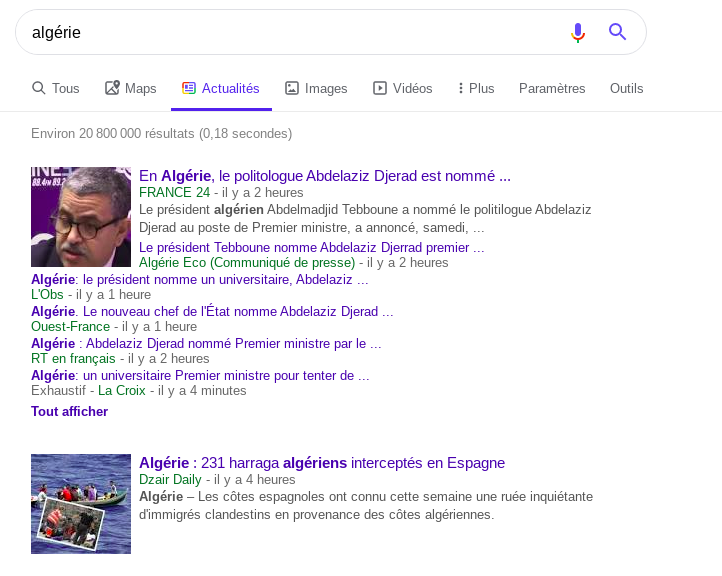
\includegraphics[height=.87\textheight]{..//img/Bweb02-ri-gmail/google-news.png}
\end{center}

\end{frame}

\begin{frame}
\frametitle{Rechercher avec Google: Effectuer une recherche}
\framesubtitle{Services: Images}

\begin{center}
	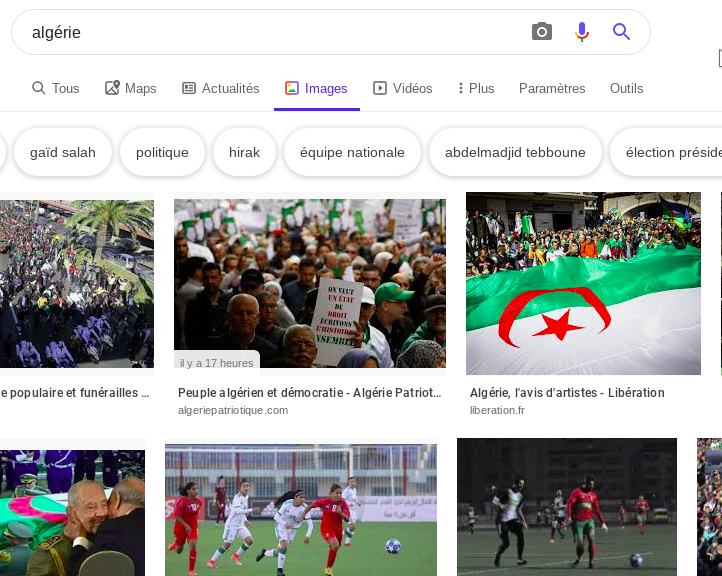
\includegraphics[height=.87\textheight]{..//img/Bweb02-ri-gmail/google-images.png}
\end{center}

\end{frame}

\begin{frame}
\frametitle{Rechercher avec Google: Effectuer une recherche}
\framesubtitle{Services: Vidéos}

\begin{center}
	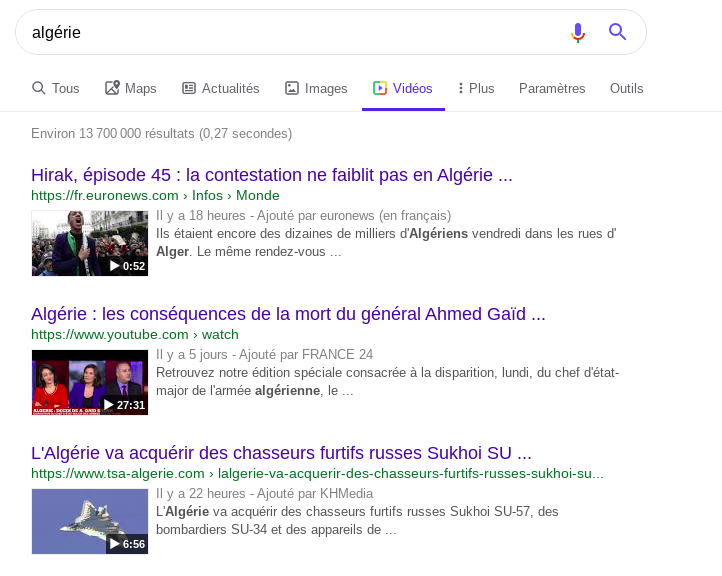
\includegraphics[height=.87\textheight]{..//img/Bweb02-ri-gmail/google-videos.png}
\end{center}

\end{frame}

\begin{frame}
\frametitle{Rechercher avec Google: Effectuer une recherche}
\framesubtitle{Services: Maps}

\begin{center}
	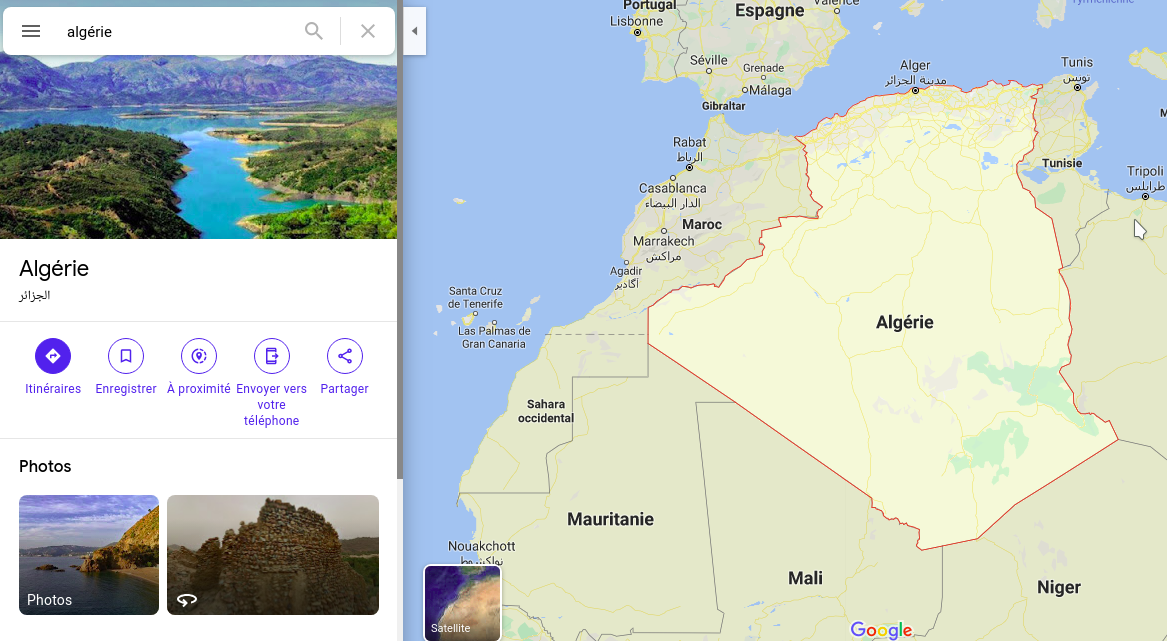
\includegraphics[height=.8\textheight]{..//img/Bweb02-ri-gmail/google-maps.png}
\end{center}

\end{frame}

\begin{frame}
\frametitle{Rechercher avec Google: Effectuer une recherche}
\framesubtitle{Les opérateurs de recherche}

% https://support.google.com/websearch/answer/2466433?hl=fr
\scriptsize\bfseries
\begin{tabular}{p{.2\textwidth}p{.25\textwidth}p{.45\textwidth}}
	
	\hline
	Opération & Exemple & Explication \\
	\hline 
	
	Rechercher plusieurs mots & université algérie & 
	Trouver les pages contenant \textcolor{red}{université} et \textcolor{red}{algérie} quelque soit l'ordre d'apparition \\
	\hline
	
	Rechercher un mot ou un autre & université \textcolor{red}{OR} algérie & 
	Trouver les pages contenant soit \textcolor{red}{université} ou \textcolor{red}{algérie} et pas les deux \\
	\hline
	
	Rechercher une correspondance exacte & \textcolor{red}{"}université en algérie\textcolor{red}{"} & 
	Trouver les pages contenant cette expression telle qu'elle est \\
	\hline
	
	Exclure des mots de votre recherche & université \textcolor{red}{-}algérie & 
	Trouver les pages contenant \textcolor{red}{université} et ne contenant pas \textcolor{red}{algérie}\\
	\hline
	
	Rechercher dans une plage de nombres & smartphone 150000\textcolor{red}{..}200000 dzd & 
	Trouver les pages contenant un nombre entre \textcolor{red}{150000} et \textcolor{red}{200000} en plus des deux autres mots\\
	\hline
	
	Rechercher un site spécifique & admis \textcolor{red}{\NoAutoSpacing site:}esi.dz & 
	Trouver les pages contenant \textcolor{red}{admis} dans le site web \textcolor{red}{esi.dz} \\
	\hline
	
	Rechercher un format spécifique & réseaux \textcolor{red}{\NoAutoSpacing filetype:}pdf & 
	Trouver les fichiers pdf contenant le mot \textcolor{red}{réseaux}\\
	\hline
	
	
\end{tabular}


\end{frame}


\subsection{Paramètres et outils de recherche}

\begin{frame}
\frametitle{Rechercher avec Google}
\framesubtitle{Paramètres et outils de recherche}

\begin{center}
	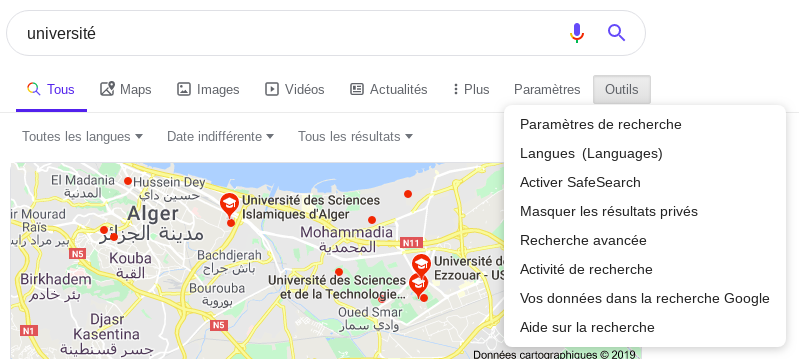
\includegraphics[width=\textwidth]{..//img/Bweb02-ri-gmail/google-param-outil.png}
\end{center}

\end{frame}

\begin{frame}
\frametitle{Rechercher avec Google: Paramètres et outils}
\framesubtitle{Paramètres: Langue}

\begin{center}
	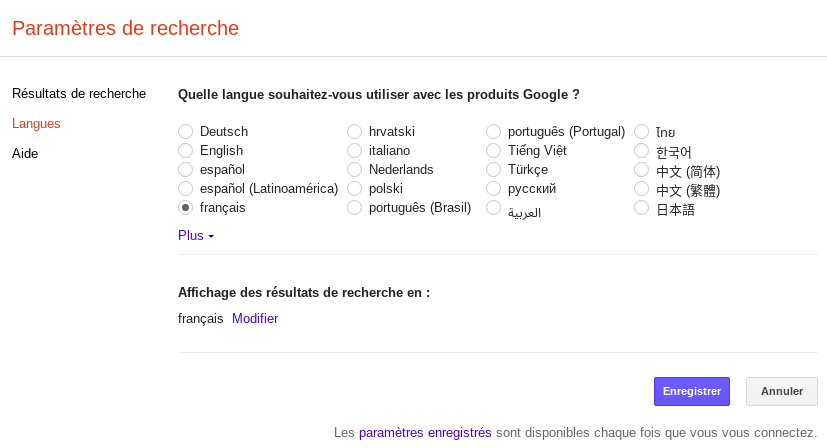
\includegraphics[height=.87\textheight]{..//img/Bweb02-ri-gmail/google-param-lang.png}
\end{center}

\end{frame}

\begin{frame}
\frametitle{Rechercher avec Google: Paramètres et outils}
\framesubtitle{Paramètres: Recherche avancée}

\begin{center}
	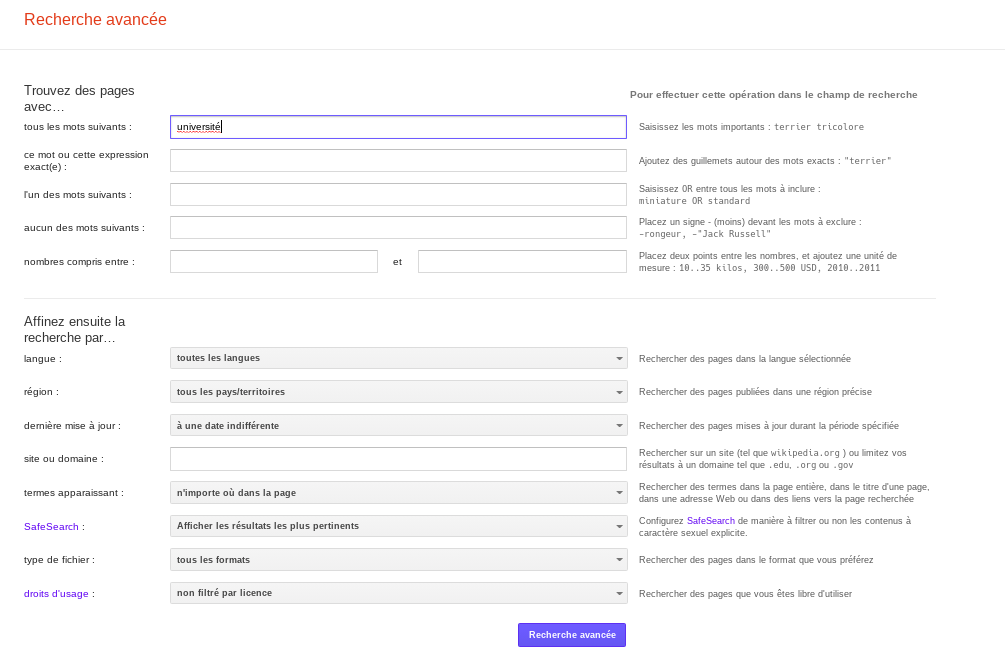
\includegraphics[height=.87\textheight]{..//img/Bweb02-ri-gmail/google-param-avance.png}
\end{center}

\end{frame}

\begin{frame}
\frametitle{Rechercher avec Google: Paramètres et outils}
\framesubtitle{Paramètres: Activité de recherche}

\begin{center}
	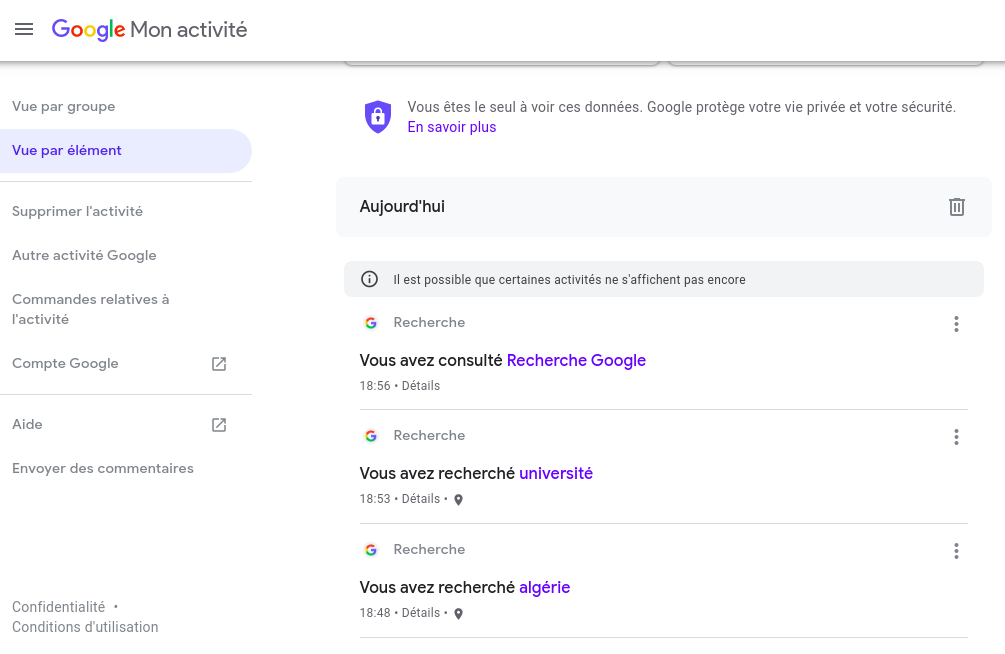
\includegraphics[height=.87\textheight]{..//img/Bweb02-ri-gmail/google-param-activite.png}
\end{center}

\end{frame}

\begin{frame}
\frametitle{Rechercher avec Google: Paramètres et outils}
\framesubtitle{Outils}

\begin{tabular}{llll}
	
	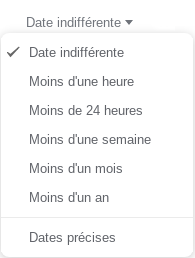
\includegraphics[width=2cm]{..//img/Bweb02-ri-gmail/google-outils-date.png} &
	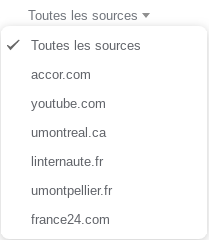
\includegraphics[width=2cm]{..//img/Bweb02-ri-gmail/google-outils-source.png} &
	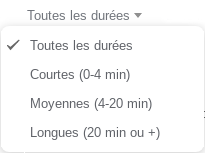
\includegraphics[width=2cm]{..//img/Bweb02-ri-gmail/google-outils-duree.png} &
	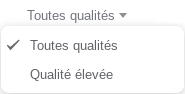
\includegraphics[width=2cm]{..//img/Bweb02-ri-gmail/google-outils-qualite.png} \\
	
	Tous &
	Vidéos &
	Vidéos &
	Vidéos \\
	
	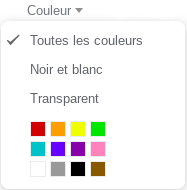
\includegraphics[width=2cm]{..//img/Bweb02-ri-gmail/google-outils-couleur.png} &
	
\includegraphics[width=2cm]{..//img/Bweb02-ri-gmail/google-outils-type.png} &
	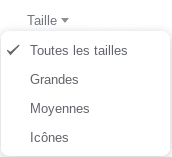
\includegraphics[width=2cm]{..//img/Bweb02-ri-gmail/google-outils-taille.png} &
	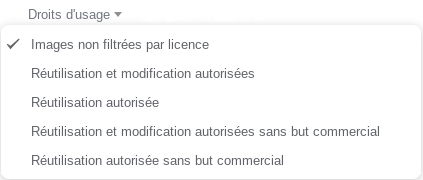
\includegraphics[width=4cm]{..//img/Bweb02-ri-gmail/google-outils-droit.png} \\
	
	Images &
	Images &
	Images &
	Images \\
	
\end{tabular}

\end{frame}

\subsection{Services supplémentaires}

\begin{frame}
\frametitle{Rechercher avec Google}
\framesubtitle{Services supplémentaires}

En plus de la recherche, Google offre d'autres services:
\begin{itemize}
	\item Auto-complétion
	\item Calculatrice 
	\item Convertisseur d'unités
	\item Météo 
\end{itemize}

\end{frame}

\begin{frame}
\frametitle{Rechercher avec Google: Services supplémentaires}
\framesubtitle{Services supplémentaires: Auto-complétion}

\begin{center}
	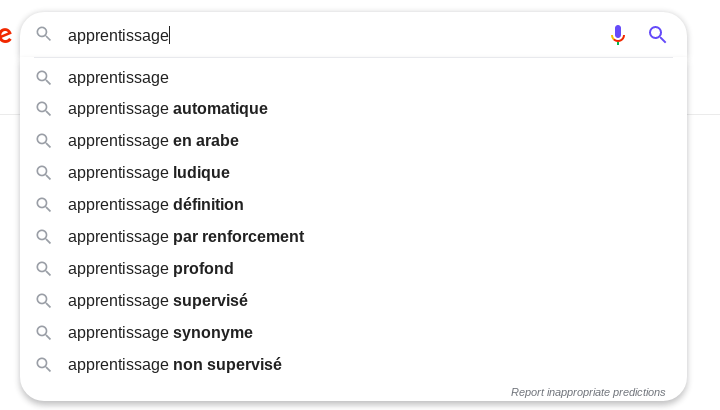
\includegraphics[height=.87\textheight]{..//img/Bweb02-ri-gmail/google-autocomplete.png}
\end{center}

\end{frame}

\begin{frame}
\frametitle{Rechercher avec Google: Services supplémentaires}
\framesubtitle{Services supplémentaires: Calculatrice}

\begin{center}
	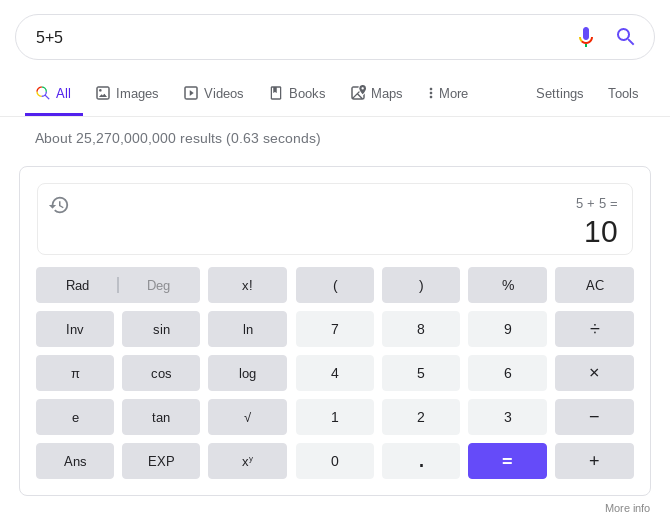
\includegraphics[height=.87\textheight]{..//img/Bweb02-ri-gmail/google-calc.png}
\end{center}

\end{frame}

\begin{frame}
\frametitle{Rechercher avec Google: Services supplémentaires}
\framesubtitle{Services supplémentaires: Convertisseur d'unités (ex. devises)}

\begin{center}
	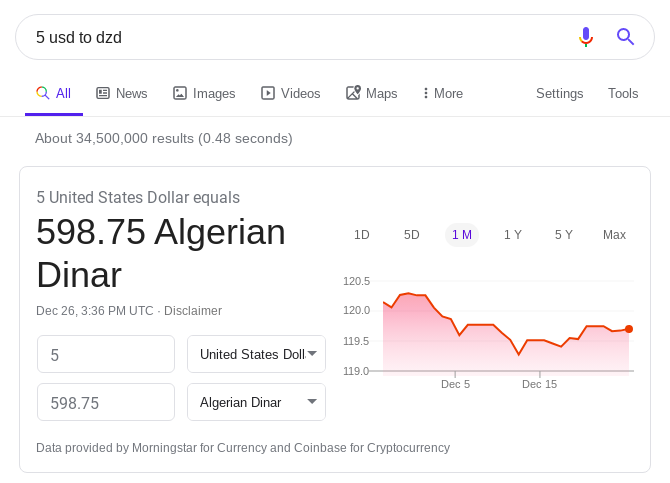
\includegraphics[height=.87\textheight]{..//img/Bweb02-ri-gmail/google-money.png}
\end{center}

\end{frame}

\begin{frame}
\frametitle{Rechercher avec Google: Services supplémentaires}
\framesubtitle{Services supplémentaires: Météo}

\begin{center}
	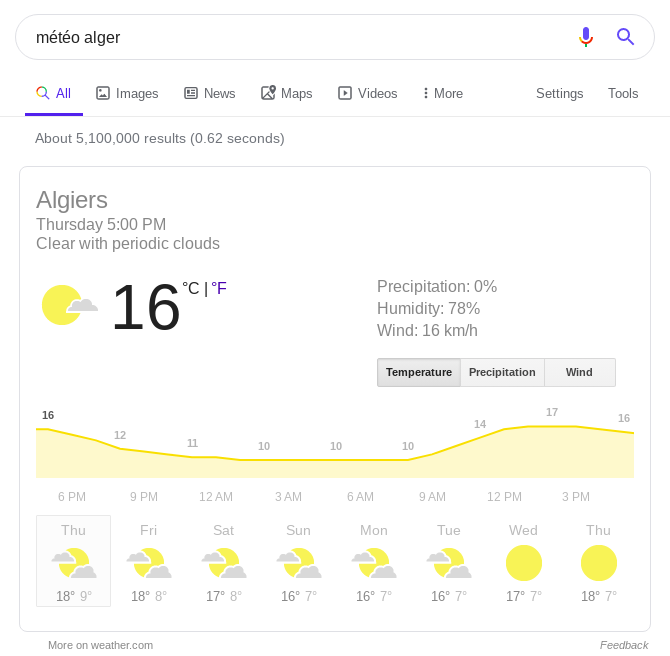
\includegraphics[height=.87\textheight]{..//img/Bweb02-ri-gmail/google-weather.png}
\end{center}

\end{frame}

\section{Messagerie électronique}

\begin{frame}
\frametitle{Messagerie électronique}

\end{frame}

\begin{frame}
\frametitle{Messagerie électronique}
\framesubtitle{Aspect légal en Algérie}


\begin{block}{Article 323 du code civil}
	L'écrit sous forme électronique est admis en tant que preuve au même titre que l'écrit sur support papier, à la condition que puisse être dûment identifiée la personne dont il émane et qu’il soit établi et conservé dans des conditions de nature à en garantir l'intégrité.
\end{block}

Un message électronique est une preuve, si on peut prouver: 
\begin{itemize}
	\item ...: on peut identifier l'expéditeur 
	\item Intégrité: le message n'a pas été modifié 
\end{itemize}

\end{frame}

\begin{frame}
\frametitle{Messagerie électronique}
\framesubtitle{Accès à la messagerie (Navigateur)}

\end{frame}

\begin{frame}
\frametitle{Messagerie électronique}
\framesubtitle{Accès à la messagerie (Client de messagerie)}

\end{frame}

\begin{frame}
\frametitle{Messagerie électronique}
\framesubtitle{Accès à la messagerie (comparaison)}

\begin{tabular}{p{.08\textwidth}p{.41\textwidth}p{.41\textwidth}}
	\hline\hline
	& Navigateur web & Client de messagerie \\
	\hline\hline
	
	Gain &
	+  
	
	+ 
	
	& 
	+ 
	
	+ 
	\\
	
	\hline
	Perte &
	- 
	
	- 
	&
	- 
	
	- 
	\\
	\hline\hline
\end{tabular}

\end{frame}



\section{Messagerie Gmail}

\begin{frame}
\frametitle{Messagerie Gmail}

\end{frame}



%\subsection{Bibliography}
%\frame[allowframebreaks]%
%{\frametitle{Bibliography}
%\tiny
%\bibliography{biblio}
%\bibliographystyle{apalike} 
%}


\end{document}

